%% This Beamer template is based on the one found here: https://github.com/sanhacheong/stanford-beamer-presentation, and edited to be used for Stanford ARM Lab

\documentclass[10pt]{beamer}
%\mode<presentation>{}

\usepackage[spanish]{babel}
\usepackage{media9}
\usepackage{amssymb,amsmath,amsthm,enumerate}
\usepackage[utf8]{inputenc}
\usepackage[T1]{fontenc}
\usepackage{array}
\usepackage[parfill]{parskip}
\usepackage{graphicx}
\usepackage{caption}
\usepackage{subcaption}
\usepackage{bm}
\usepackage{amsfonts,amscd}
\usepackage[]{units}
\usepackage{listings}
\usepackage{multicol}
\usepackage{multirow}
\usepackage{tcolorbox}
\usepackage{physics}
\usepackage{circuitikz}
\usepackage{wrapfig}

% Enable colored hyperlinks
%\hypersetup{colorlinks=true}

% The following three lines are for crossmarks & checkmarks
\usepackage{pifont}% http://ctan.org/pkg/pifont
\newcommand{\cmark}{\ding{51}}%
\newcommand{\xmark}{\ding{55}}%

% Numbered captions of tables, pictures, etc.
\setbeamertemplate{caption}[numbered]

%\usepackage[superscript,biblabel]{cite}
\usepackage{algorithm2e}
\renewcommand{\thealgocf}{}

% Bibliography settings
\usepackage[style=ieee]{biblatex}
\setbeamertemplate{bibliography item}{\insertbiblabel}
\addbibresource{references.bib}

% Glossary entries
\usepackage[acronym]{glossaries}
\newacronym{ML}{ML}{machine learning}
\newacronym{HRI}{HRI}{human-robot interactions}
\newacronym{RNN}{RNN}{Recurrent Neural Network}
\newacronym{LSTM}{LSTM}{Long Short-Term Memory}


\theoremstyle{remark}
\newtheorem*{remark}{Remark}
\theoremstyle{definition}

\newcommand{\empy}[1]{{\color{darkorange}\emph{#1}}}
\newcommand{\empr}[1]{{\color{cardinalblue}\emph{#1}}}
\newcommand{\examplebox}[2]{
  \begin{tcolorbox}[colframe=darkcardinal,colback=boxgray,title=#1]
	#2
\end{tcolorbox}}

\usetheme{Stanford} 
\input{./style_files_stanford/my_beamer_defs.sty}

% commands to relax beamer and subfig conflicts
% see here: https://tex.stackexchange.com/questions/426088/texlive-pretest-2018-beamer-and-subfig-collide
\makeatletter
\let\@@magyar@captionfix\relax
\makeatother

\title[Proyecto Final]{Estudio e Implementaci\'on de un Sistema de
Administraci\'on de Bater\'ias de Li-Ion de baja y mediana potencia.}
\subtitle{Presentación final - Proyecto I}

%\beamertemplatenavigationsymbolsempty

\begin{document}

\institute{
  \vskip 5pt
  \begin{figure}
	\centering
	\begin{subfigure}[t]{0.5\textwidth}
	  \centering
	  \includegraphics[height=0.7in]{./images/LOGO-UNR-NEGRO.png}
	\end{subfigure}%
	~ 
	\begin{subfigure}[t]{0.5\textwidth}
	  \centering
	  \includegraphics[height=0.5in]{./images/FCEIA-logo.png}
	\end{subfigure}
  \end{figure}
  \vskip 5pt
  Facultad de Ciencias Exactas, Ingeniería y Agrimensura\\
  Universidad Nacional de Rosario\\
  \vskip 1pt
}

\author[Escuela de Ingeniería Electrónica]{
  \begin{tabular}{ccc} 
	Federico Ceccarelli & Martin Moya & Lucio Santos\\
	\footnotesize
	\texttt{\href{mailto:fededc88@gmail.com}{fededc88@gmail.com}} &
	\footnotesize
	\texttt{\href{mailto:moyamartin1@gmail.com}{moyamartin1@gmail.com}} &
	\footnotesize
	\texttt{\href{mailto:lucio.santos2206@gmail.com}{lucio.santos2206@gmail.com}}
  \end{tabular}
\vspace{-4ex}}

\date{\today}

\begin{noheadline}
  \begin{frame}\maketitle\end{frame}
\end{noheadline}

\setbeamertemplate{itemize items}[default]
\setbeamertemplate{itemize subitem}[circle]

\begin{frame}%[allowframebreaks]
	\frametitle{Contenidos} % Table of contents slide, comment this block out to remove it
    \small
	\tableofcontents % Throughout your presentation, if you choose to use \section{} and \subsection{} commands, these 	will automatically be printed on this slide as an overview of your presentation
\end{frame}

\section{Objetivos del proyecto}

\begin{frame}[allowframebreaks]
    \frametitle{Objetivos del proyecto}

    En el presente trabajo se detalla el proceso de investigaci\'on, desarrollo e
    implementaci\'on de un administrador de bater\'ias, tambien conocido como BMS (del
    ingl\'es Battery Management System), compatible con un pack de bater\'ias de iones
    de litio.

    \vspace{10mm}

    \begin{figure}[h!]
        \includegraphics[width=1\textwidth]{./images/db_bms.png}
        \caption{Diagrama en Bloques del BMS y el pack de bater\'ia}
        \label{fig:r_ohm_result}
    \end{figure}

    \newpage

    \textbf{Objetivos BSM:}
    \begin{itemize}
        \item Proteger el pack de bater\'ias evitando que el mismo salga de su
            zona de operaci\'on segura.
        \item Estimar el estado de carga (\emph{SoC}) en tiempo real.
        \item Balancear la carga entre celdas.
        \item Comunicar los par\'ametros fundamentales del pack.
    \end{itemize}
\end{frame}

\section{Estimación del SoC}

\subsection{Métodos de estimación}
\begin{frame}[allowframebreaks]
	\frametitle{Métodos de Estimación de SoC}
  	Hoy en día hay varios métodos para estimar el Estado de Carga de una batería,
  	entre ellas se encuentran las siguientes:
  	\begin{itemize}
        \item Metodos Tradicionales
            \begin{itemize}
                \item 	Relación directa entre el SoC y el OCV
                \item 	Integración de Corriente \emph{Coulomb Counting}.
                \item 	Resistencia Interna.
            \end{itemize}
        \item Metodos Modernos
            \begin{itemize}
                \item 	\textbf{Estimación del Estado de Carga basado en la Teor\'ia de
                    Control y modelos matemáticos.}
                \item 	Metodos basados en IA y Aprendizaje Automático.
            \end{itemize}
  	\end{itemize}
	\framebreak
  	Dentro del último, nos encontramos con los distintos modelos disponibles:
  	\begin{itemize}
		\item	Estimación basada en modelos Térmico y Electroquímicos.
		\item	Modelo Eléctrico.
	  % TODO: Mover espectroscopía dieléctrica.
		\item 	Espectroscopía Dielétrica.
  	\end{itemize}
  	El error inherente de estos modelos puede ser compensado utilizando Filtros
  	predictivos, como por ejemplo, un Filtro de Kalman con sus respectivas
  	variaciones.
\end{frame}


\begin{frame}[allowframebreaks]
    \frametitle{ M\'etodo de c\'alculo del SoC implementado.}
    Implementamos  un modelo eléctrico de una celda de Litio-Ion complementado
    con un Filtro de Kalman debido a que:
  	\begin{itemize}
		\item Los componentes eléctricos de un modelo y sus dinámicas ya son de
	  		de nuestro conocimiento y f\'aciles de simular.
		\item Los c\'alculos de los parámetros del circuito son simples de estimar en
	  		base a un set de datos.
        \item El Filtro de Kalman es un filtro predictor con amplia
            bibliograf\'ia y ejemplos, lo que facilita su implementación.
		\item La complejidad computacional tanto del modelo el\'ectrico como el filtro
	 		de Kalman son bajos.
		\item Nos permite extender el modelo a una implementación f\'isica con un
	  		ajuste fino minimizando errores.
  	\end{itemize}
\end{frame}

\subsection{Modelo equivalente}
\begin{frame}
	\frametitle{Datos Experimentales}
	Como punto de partida, utilizamos un set de datos 
	%TODO: agregar referencia a bibtex del dataset
	de la Universidad de Wisconsin-Madison donde se realizó una serie de 
	ensayos sobre una celda NCR18650P. En la figura \ref{fig:perfildeensayohppc},
	se puede observar un ensayo HPPC sobre la celda.
  	\begin{figure}
		\centering
		\includegraphics[width=1\linewidth]{images/HPPC-Completo}
		\caption{Perfil V-I de ensayo HPPC completo}
		\label{fig:perfildeensayohppc}
   	\end{figure}
\end{frame}

\begin{frame}[allowframebreaks]
	\frametitle{Modelo equivalente de una celda NCR18650PF}
  	El modelo equivalente propuesto para replicar la dinámica de la celda a
  	implementar se puede observar en la figura \ref{fig:ModeloBat}
  	\begin{figure}
		\begin{center}
	  	\resizebox{0.40\textwidth}{!}{%
	  	\ctikzset{bipoles/length=1cm}
	  	\begin{circuitikz}[american]
			\draw (0,3) to[vsource, v=$V_{m}$](0,0);
			\draw (0,3) to [R = $R_{0}$](2,3);
			\draw (2,2.5)--(2,3.5);
			\draw (2,3.5) to [C=$C_{1}$] (4,3.5);
			\draw (2,2.5) to [R=$R_{1}$] (4,2.5);
			\draw (4,2.5)--(4,3.5);
			\draw (4,3) -- (5,3);
			\draw (5,2.5)--(5,3.5);
			\draw (5,3.5) to [C=$C_{2}$] (7,3.5);
			\draw (5,2.5) to [R=$R_{2}$] (7,2.5);
			\draw (7,2.5)--(7,3.5);
			\draw (7,3) -* (9,3);
			\draw (7,3) to[short,i^=$I$] (9,3)
			to[open,v^=$v_{term}$,o-o] (9,0)
			to[short] (0,0);
	  	\end{circuitikz}
	  	}%
	  \caption{Modelo equivalente celda NCR18650B}
	  \label{fig:ModeloBat}
	  \end{center}
	\end{figure}
	\begin{minipage}{0.45\linewidth}
  		Validamos el orden del modelo gráficamente ajustando una función 
  		suma de exponenciales, como \ref{eq:exp2}, a la evolución del 
  		voltaje en terminales de la bateria en su semi-periodo de relajación.
  		\begin{equation}
			f(x) = a*e^{b*x} + c*e^{d*x}
			\label{eq:exp2}
  		\end{equation}
	\end{minipage}\hfill
	\begin{minipage}{0.45\linewidth}
  		\begin{figure}[h!]
			\centering
			\includegraphics[width=1.3\linewidth]{images/exp_ord_2_val.png}
			\caption{Validación del modelo}
			\label{fig:val_exp2}
  		\end{figure}
	\end{minipage}
\end{frame}

\begin{frame}[allowframebreaks]
	\frametitle{Estimación de parámetros del modelo}
  	Implementamos en Matlab un estimador de parámetros RC del 
  	modelo propuesto. Usamos el\emph{Estimador de parámetros} del Toolbox 
  	Identificador de Sistemas de simulink.\\
  	El método implementado es el de aproximaciones sucesivas a partir de comparar 
  	los datos experimentales con los obtenidos a partir de la simulación de 
  	simulink.
  	\begin{figure}[!hb]
		\centering
		\includegraphics[width=0.9\linewidth]{images/battery_model_simulink.png}
		\caption{Modelo Simulink Simscape de celda  NCR18650B }
		\label{fig:simulink_celda}
  	\end{figure}
  	Fraccionamos los datos experimentales obtenidos del ensayo HPPC y calculamos/ajustamos
  	un juego de parámetros para cada escalon de corriente del ensayo asociado a 
  	un SOC determinado.
  	\begin{figure}[!hb]
		\centering
		\includegraphics[width=0.9\linewidth]{images/Optimizacion.png}
		\caption{Resultado proceso Ajuste de parametros del modelo}
		\label{fig:RC_Opt}
  	\end{figure}
  	\framebreak
  	Obtuvimos 67 juegos de valores internos del modelo para 67 estados de carga distintos.\\
  	Corregimos los valores obtenidos sometiendo el modelo calculado a multiples 
  	perfiles de corriente de distintos drive cicles y comparando los datos obtenidos con 
  	los valores experimentales.
  	\begin{figure}[!h]
		\centering
		\includegraphics[width=0.85\linewidth]{images/Drive_Cicle_Modelo_Bateria.png}
		\caption{Drive Cicle - Modelo Vs Data}
		\label{fig:DC_modVsData}
  	\end{figure}
\end{frame}

\subsection{Filtro de Kalman}

\begin{frame}[allowframebreaks]
  	\frametitle{Filtro de Kalman}
  	El filtro de Kalman es un algoritmo recursivo que corrige las estimaciones
  	mediante la probabilidad conjunta de una o varias mediciones de un fenómeno y
  	su estimación obtenida por modelos matemáticos.
  	\begin{figure}[h!]
		\centering
		\includegraphics[width=0.7\textwidth]{images/KalmanFilterDiagram.png}
		\caption{Diagrama del Filtro de Kalman}
		\label{fig:kf_sch}
  	\end{figure}
\end{frame}

\begin{frame}[allowframebreaks]
  \frametitle{Filtro de Kalman - Objetivos}
  El filtro de Kalman logra que la estimación del SoC sea robusta ante:
  \begin{itemize}
	\item Valor de SoC inicial incorrecto.
	\item Ruido y offset en las mediciones.
	\item Dispersión paramétrica entre celdas del mismo fabricante.
  \end{itemize}
  Como fundamento teórico, requiere que el sistema sea modelado en un sistema de
  ecuaciones de estado, como el de la siguiente forma:

  \begin{align*}
	\dot{x} = Ax + Bu \\
	y = Cx + Du
	\label{sse}
  \end{align*}

  \framebreak

  Donde, para el modelo desarrollado, obtenemos que:

  \begin{align*}
	\dot{x} = \begin{bmatrix} 
	  v_1\\
	  v_2\\
	  SoC
	\end{bmatrix}
	\qquad
	y = v
  \end{align*}
  \begin{align*}
	A = \begin{bmatrix}
	  -\frac{1}{R_1(SoC)C_1(SoC)} & 0 & 0\\
	  0 & -\frac{1}{R_2(SoC)C_2(SoC)} & 0\\
	  0 & 0 & 0
	\end{bmatrix}
	\qquad
	B = \begin{bmatrix}
	  \frac{1}{C_1(SoC)}\\
	  \frac{1}{C_2(SoC)}\\
	  -\frac{1}{S_{c, a}}
	\end{bmatrix}
  \end{align*}
  \begin{align*}
	C = \begin{bmatrix} -1 & -1 & V_{OCV}(SoC)\end{bmatrix} \qquad D = -R_0(SoC)
  \end{align*}
  \framebreak
	
  El algoritmo también requiere de las siguientes definiciones:
  \begin{itemize}
	\item \textbf{Matriz de incerteza en la medición (R)}: Esta incerteza se
	  encuentra directamente relacionada con los sensores involucrados
	  (corriente y tensión).
	\item \textbf{Incerteza del ruido en el proceso (Q)}: Relacionado
	  directamente a las aspectos no lineales del sistema como también
	  perturbaciones externas (temperatura, estado de salud, etc).
	\item \textbf{Valores iniciales del sistema}: El filtro requiere
	  un estado inicial y una incerteza del mismo.
  \end{itemize}
\end{frame}

\subsection{Resultados y Observaciones}
\begin{frame}[allowframebreaks]
  \frametitle{Resultados y Observaciones}
  \begin{figure}[h!]
	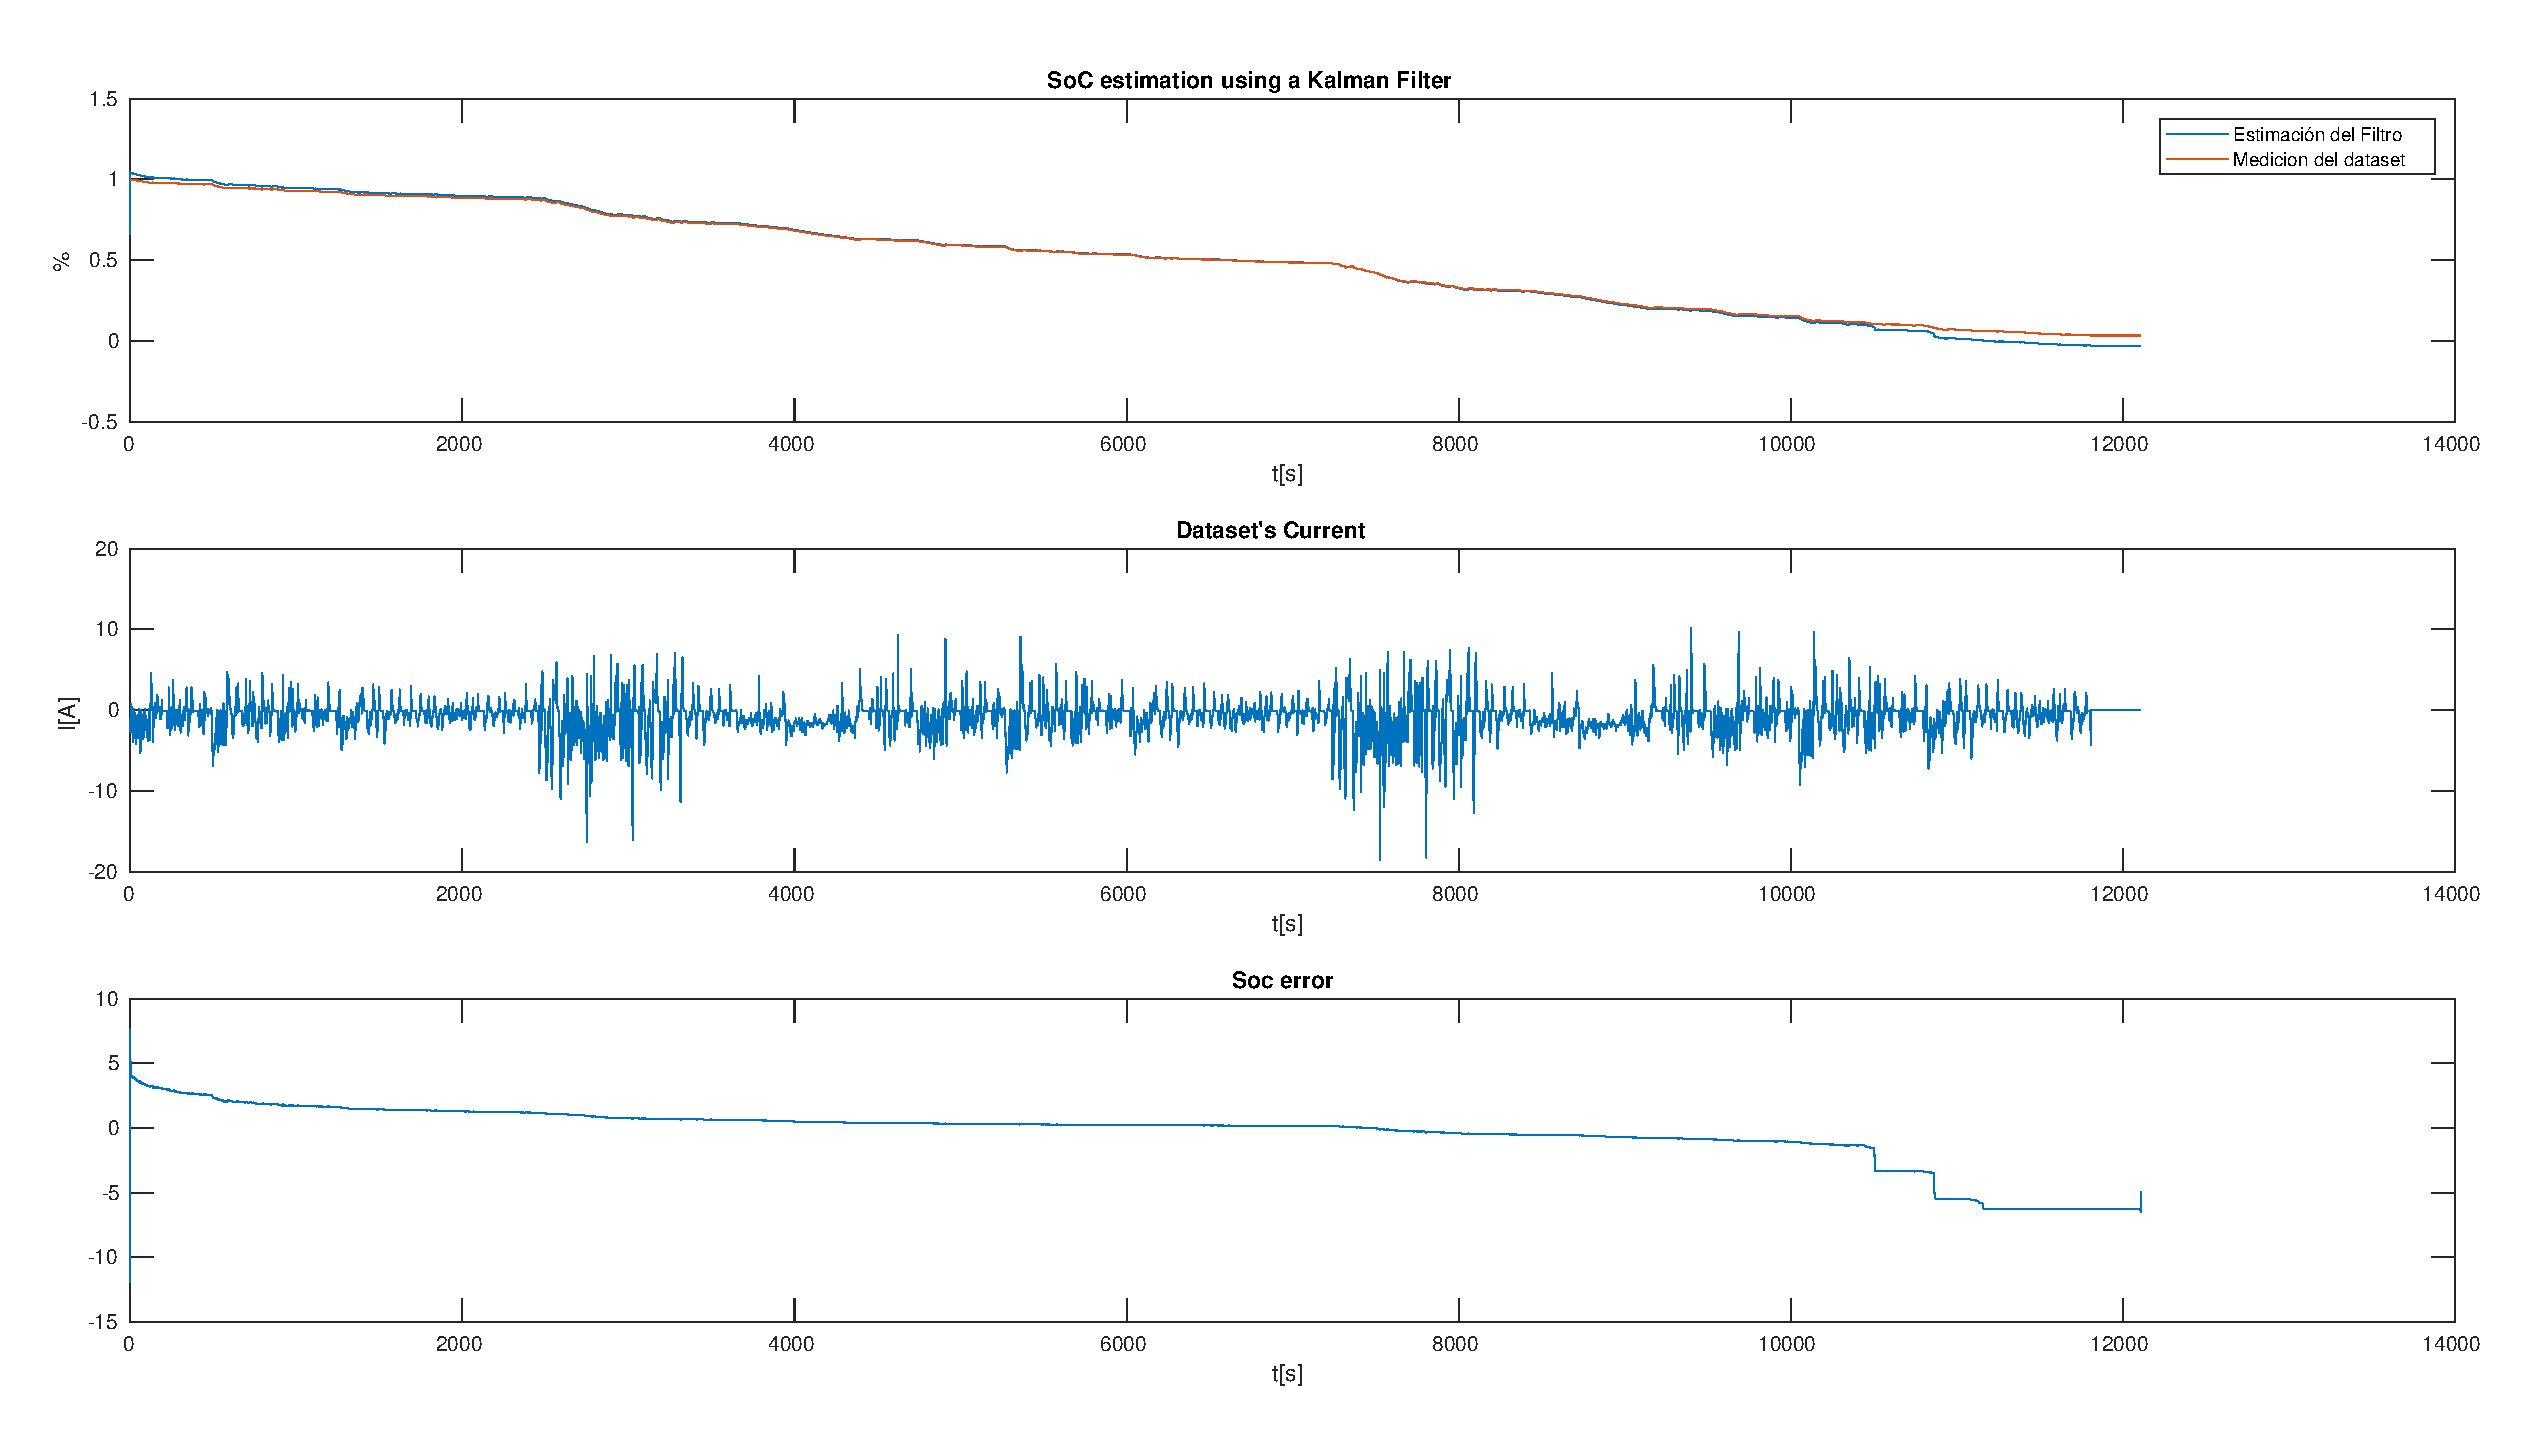
\includegraphics[width=1\textwidth]{images/kf_result_25degree.eps}
  \end{figure}
\end{frame}

\section{Hardware}

\begin{frame}
	\frametitle{Desarrollo del Hardware}
    Se seleccionaron los componenetes y se estudiaron e implementarons los
    circuitos de los subsistemas del BMS, los mismos son:

  	\begin{minipage}{0.4\textwidth}
		\small
		\begin{itemize}
            \item Unidad de procesamiento
	  		\item Alimentaci\'on CPU
	  		\item Balanceador y Sensor de Tensi\'on
	 		\item Sensor de Corriente
		\end{itemize}
 	 \end{minipage}
  	\hfill
  	\begin{minipage}{0.4\textwidth}
		\small
		\begin{itemize}
            \item Interruptor de Seguridad entre Bater\'ia y Veh\'iculo
	  		\item Pack de bater\'ias
	 		\item Puerto de Comunicaci\'on
	  		%\vspace{4\baselineskip}
		\end{itemize}
  	\end{minipage}
  	\begin{figure}[h!]
	  		\centering
            \includegraphics[width=0.75\linewidth]{images/db_hardware.png}
	  		\caption{DB Hardware BMS}
  	\end{figure}
\end{frame}

\begin{frame}
    \frametitle{Circuito Impreso Final}

    \begin{figure}[h!]
        \begin{center}
            \includegraphics[width=0.8\textwidth]{images/render_pcb.png}
            \caption{Renderizado 3D del circuito impreso final, solo se muestra la
            cara superior de la placa.}
            \label{render_pcb}
        \end{center}
    \end{figure}
\end{frame}

\begin{frame}
    \frametitle{Foto BMS}
    \begin{figure}[h!]
        \begin{center}
            \includegraphics[width=0.8\textwidth]{images/placa_bms_foto.png}
            \caption{Foto tomada despu\'es de finalizar el ensamblado y los ensayos
                finales, se pueden notar conexiones soldadas para arreglar errores de
            diseño.}
            \label{placa_bms_fotografia}
        \end{center}
    \end{figure}
\end{frame}

\subsection{Unidad de Procesamiento}
\begin{frame}
    \frametitle{Unidad de Procesamiento}

    \begin{wrapfigure}{R}{2.5cm}
        \includegraphics[width=2.5cm]{images/STM32F407VG.png}
        \caption{STM32f407VG}
        \label{fig:stm32f407vg}                                                            
    \end{wrapfigure}                                                                 

    \textbf{STM STM32F407VG:}\\
    La naturaleza de los desafios matemáticos que plantea el desarrollo del BMS y el
    rendimiento computacional requerido para el procesamiento en tiempo real fueron
    dos de los pilares fundamentales para la selección e implementación del
    Microcontrolador STM32F407VG de la empresa STMicroelectronics.

    \textbf{TI TPS54331:}\\
    Para alimentar la unidad de procesamiento del BMS se desarrolla e implementa
    un convertidor de tensión DC-DC basado en el circuito integrado TPS54331 de
    tecnolog\'ia switching tipo Step Down de la firma Texas Instruments

\end{frame}

\subsection{Sensor de Tensión - Balanceador}
\begin{frame}
    \frametitle{Sensor de Tensión - Balanceador}

    \begin{wrapfigure}{R}{2.5cm}
        \includegraphics[width=2.5cm]{images/bq76_simplified_schematic.png}
        \caption{STM32f407VG}
        \label{fig:stm32f407vg}                                                            
    \end{wrapfigure}                                                                 

    Se opt\'o por un criterio de balanceo basado en una topolog\'ia pasiva
    utilizando resistencias shunt en conjunto con una estrategia de control
    cl\'asica que depende del promedio del SoC entre las 6 celdas, estableciendo
    un umbral m\'aximo de variación entre celdas como criterio de balanceo.

    \textbf{TI BQ76PL536A:}\\
    El dispositivo es un monitor y protector de bater\'ias compuestos por 3 a 6
    celdas conectadas en serie, que pueden acoplarse entre s\'i para extenderse
    a 192 celdas. Integra un frontend anal\'ogico (AFE, del ingl\'es
    Analog Frontend) en conjunto con un conversor analógico-digital (ADC, del
    ingl\'es Analog-to-digital con- verter), utilizado para medir de forma precisa
    el voltaje de cada celda.

\end{frame}

\subsection{Pack de Bater\'ias}
\begin{frame}
    \frametitle{Pack de Bater\'ias}

    Durante el proceso de desarrollo del BMS implementamos nuestro propio pack
    de baterc\'ias con el objetivo de que el mismo cumpla con las especificaciones
    necesarias que nos permitan llevar adelante los ensayos plateados.

    \begin{figure}[h!]
        \begin{subfigure}[b]{.5\textwidth}
            \begin{center}
                \begin{minipage}[c]{0.45\textwidth}
                    \centering
                    \begin{circuitikz}[european, scale = 0.5, transform shape]

                        \draw (7, 2) -- (7, 2.2);
                        \draw (7, 2) to[battery1] (7, 1.6);
                        \draw (7, 1.4) -- (7, 1.6);
                        \draw (7, 1.4) to[battery1] (7, .9);			
                        \draw (7, .7) -- (7, .9);			
                        \draw (7, 0.7) to[battery1] (7, 0.2);			
                        \draw (7, 0.2) -- (7, -0.2);
                        \draw (7, -0.2) to[battery1] (7, -0.7);
                        \draw (7, -.7) -- (7, -.9);
                        \draw (7, -.9) to[battery1] (7, -1.4);
                        \draw (7, -1.4) -- (7, -1.6);
                        \draw (7, -1.6) to[battery1] (7, -2);
                        \draw (7, -2) -- (7, -2.2);

                        \draw (9, 2) -- (9, 2.2);
                        \draw (9, 2) to[battery1] (9, 1.6);
                        \draw (9, 1.4) -- (9, 1.6);
                        \draw (9, 1.4) to[battery1] (9, .9);			
                        \draw (9, .7) -- (9, .9);			
                        \draw (9, 0.7) to[battery1] (9, 0.2);			
                        \draw (9, 0.2) -- (9, -0.2);
                        \draw (9, -0.2) to[battery1] (9, -0.7);
                        \draw (9, -.7) -- (9, -.9);
                        \draw (9, -.9) to[battery1] (9, -1.4);
                        \draw (9, -1.4) -- (9, -1.6);
                        \draw (9, -1.6) to[battery1] (9, -2);
                        \draw (9, -2) -- (9, -2.2);

                        \draw (11, 2) to[battery1] (11, 1.6);
                        \draw (11, 1.4) -- (11, 1.6);
                        \draw (11, 1.4) to[battery1] (11, .9);			
                        \draw (11, .7) -- (11, .9);			
                        \draw (11, 0.7) to[battery1] (11, 0.2);		
                        \draw (11, 0.2) -- (11, -0.2);
                        \draw (11, -0.2) to[battery1] (11, -0.7);
                        \draw (11, -.7) -- (11, -.9);
                        \draw (11, -.9) to[battery1] (11, -1.4);
                        \draw (11, -1.4) -- (11, -1.6);
                        \draw (11, -1.6) to[battery1] (11, -2);
                        \draw (11, -2) -- (11, -2.2);

                        \draw (7, 0) -- (9, 0);
                        \draw (9, 0) -- (11, 0);

                        \draw (7, 0.8) -- (9, 0.8);
                        \draw (9, 0.8) -- (11, 0.8);

                        \draw (7, 1.5) -- (9, 1.5);
                        \draw (9, 1.5) -- (11, 1.5);

                        \draw (7, 2.2) -- (9, 2.2);
                        \draw (9, 2.2) -- (11, 2.2);			

                        \draw (7, -0.8) -- (9, -0.8);
                        \draw (9, -0.8) -- (11, -0.8);

                        \draw (7, -1.5) -- (9, -1.5);
                        \draw (9, -1.5) -- (11, -1.5);

                        \draw (7, -2.2) -- (9, -2.2);
                        \draw (9, -2.2) -- (11, -2.2);			

                        \draw [dashed] (6.5, 2.4) rectangle (11.5, -2.4);

                        \draw node at (8.2, 2.6) {Pack de Baterías 6s3p};
                    \end{circuitikz}
                \end{minipage}
            \end{center}
            \caption{Esquemático de la arquitectura del pack de baterías.}
            \label{pack_bateria}
        \end{subfigure}%
        \begin{subfigure}[b]{.45\textwidth}
            \centering
            \includegraphics[width=0.5\textwidth]{images/18650.jpg}
            \caption{Foto celda NCR18650PF.}
            \label{foto_bateria}
        \end{subfigure}
        \caption{Pack 6s3p y Celda NCR18650PF.}
        \label{pack}
    \end{figure}
\end{frame}

\subsection{Celda de Litio-Ion NCR18650PF}

\begin{frame}
	\frametitle{Celda NCR18650PF}
  	\vspace{10pt}
  	\begin{figure}[h!]
		\begin{minipage}{0.3\textwidth}
	  		\centering
	  		\includegraphics[width=0.45\linewidth]{images/18650}
	  		\caption{Celda NCR18650PF}
		\end{minipage}
		\begin{minipage}{0.65\linewidth}
	  		\begin{itemize}
				\item	Capacidad: \\Min. 2750mAh | Max. 2900mAh
				\item	Voltage nominal: 3.6V
				\item	Carga: CC-CV, Std. 1375mA, 4.20V, 4.0 hrs
				\item	Densidad energética: \\577Wh/l | 207 Wh/kg
	  		\end{itemize}
		\end{minipage}
  	\end{figure}
  	\vspace{10pt}
  	\begin{figure}[h!]
		\centering
		\includegraphics[width=.32\textwidth]{images/cc_cv_18650}\hfill
		\includegraphics[width=.32\textwidth]{images/discharge_18650}\hfill
		\includegraphics[width=.32\textwidth]{images/life_cycle_18650}
		\caption{Curvas características de la celda NCR18650PF}
  	\end{figure}
\end{frame}

\begin{frame}
    \frametitle{Pack de Bater\'ias}

    Como resultado obtenemos un pack de bater\'ias con las siguientes
    caracter\'isticas:
    \small
    \begin{itemize}
        \item Voltaje nominal de salida: 21.6V
        \item Voltaje m\'aximo de salida: 25.2V
        \item Voltaje m\'inimo de salida: 15V
        \item Capacidad t\'ipica: 8700mAh
        \item Capacidad m\'inima: 8250mAh
        \item Corriente de carga m\'axima: 4.35A
        \item Corriente de descarga m\'axima: 17.4A (2C)
    \end{itemize}

\begin{figure}[h!]
    \begin{subfigure}[t]{.3\textwidth}
	\begin{center}
        \includegraphics[width=.3\textwidth]{images/battery_top.png}
	\end{center}
    \caption{Imagen superior del pack de bater\'ias 6s3p. 
    }
	\label{battery_top}
    \end{subfigure}%
    \begin{subfigure}[t]{.3\textwidth}
	\centering
	\includegraphics[width=.3\textwidth]{images/battery_bot.png}
	\caption{Imagen inferior del pack de bater\'ias 6s3p.}
	\label{battery_bot}
    \end{subfigure}
    \begin{subfigure}[t]{.3\textwidth}
	\centering
	\includegraphics[width=.3\textwidth]{images/batt_side.png}
	\caption{Imagen lateral del pack de bater\'ias 6s3p. En esta foto se puede
    apreciar el conector JST}
	\label{battery_side}
    \end{subfigure}
    \label{battery_pack}
    \caption{Pack debaterías 6s3p}
\end{figure}
\end{frame}

\subsection{Sensor de Corriente}

%\begin{frame}[allowframebreaks]
%	\frametitle{Sensor de Corriente}
%  	\begin{minipage}{0.4\textwidth}
%		\textbf{Objetivos}
%		\small
%		\begin{itemize}
%	  		\item Mantener al pack operando dentro del SOA.
%	  		\item Monitorear la distribución de carga entre celdas
%	  		\item Implementar y mantener un seguimiento preciso del SoC
%	  		\vspace{4\baselineskip}
%		\end{itemize}
% 	 \end{minipage}
%  	\hfill
%  	\begin{minipage}{0.4\textwidth}
%		\textbf{Tecnologías disponibles}
%		\small
%		\begin{itemize}
%	 		\item \textbf{Resistencia Shunt}
%	  		\item Transformador de Intensidad
%	  		\item \textbf{Sensor de Efecto Hall}
%	  		\item Sensor de Impedancia Magnética
%	  		\item Sensor de Magnetoresistencia Gigante
%	  		\item Sensores Ópticos
%		\end{itemize}
%  	\end{minipage}
%\end{frame}

%\begin{frame}[allowframebreaks]
%  	\frametitle{Resistencia Shunt}
%  	Calcula la corriente de forma indirecta midiendo la caída de tensión sobre
%  	una resistencia, que tiene un valor del órden de los miliohmios, al circular
%  	la corriente incógnita.\\
%  	Su esquemático se puede observar en la Figura \ref{sch_shunt}.
%	\begin{figure}[h!]
%		\begin{circuitikz}\draw
%	  		(0, 0) to[resistor=$R_{shunt}$, i_>=$I$] (6, 0)
%	  		;
%	  		\draw
%	  		(2, 0) to[short, *-] (2, 1.5)
%	 		(2, 1.5) to[voltmeter] (4, 1.5)
%	  		(4, 1.5) to[short, -*] (4, 0)
%	  		;
%		\end{circuitikz}
%		\caption{Esquemático de un sensor de corriente por resistencia shunt}
%		\label{sch_shunt}
%  	\end{figure}
%	\framebreak
%  	Características y consideraciones:
%  	\begin{itemize}
%		\item 	Alta relación de costo-efectividad, empaquetado compacto y aplicable
%	  			en mediciones tanto de corriente continua como alterna.
%		\item 	Alta frecuencia de corte (decenas de MHz).
%		\item 	Carece de aislación galvánica.
%		\item 	Alto rango de temperatura de operación.
%		\item 	La resistencia shunt presenta una inductancia intrínseca,
%	 			comprometiendo el ancho de banda y la presición
%  	\end{itemize}
%\end{frame}
%
%\begin{frame}[allowframebreaks]
%  \frametitle{Sensor de Efecto Hall}
%  \begin{figure}[h!]
%	\begin{minipage}{0.45\textwidth}
%		Sensor de efecto magnético basado en el fenómeno físico denominado \emph{Efecto Hall}.
%	  \begin{itemize}		  
%		\item Dispositivo aislado, no intrusivo.
%		\item Mide CA como CC.
%	  \end{itemize}
%	\end{minipage}
%	\hspace{10pt}
%	\begin{minipage}{0.45\textwidth}
%	  \centering
%	  \includegraphics[width=0.7\textwidth]{./images/Open-loop_Hall_Sensor.jpg}
%	  \caption{Esquemático de un sensor de Efecto Hall}
%	  \label{sch_hall}
%	\end{minipage}
%  \end{figure}
%  \textbf{Consideraciones}:
%  \begin{itemize}
%	\item Debido al efecto de saturación magnética del núcleo, posee
%	  limitaciones en picos de corriente y frecuencias menores al MHz.
%	\item Sensible a la influencia de los campos magnéticos externos.
%	\item Presenta un voltaje de offset que es poco estable y varía
%	  fuertemente a cambios de temperatura.
%  \end{itemize}
%\end{frame}

%\begin{frame}[allowframebreaks]
%  	\frametitle{Tecnología seleccionada}
%  	Dada la naturaleza del BMS, elegimos el método de medición de corriente por
%  	resistencia Shunt, ya que posee las siguientes ventajas:
%  	\begin{itemize}
%		\item 	Bajo offset y baja susceptibilidad frente a campos magnéticos externos
%	  			y variaciones de temperatura.
%		\item	Alta linealidad, mayormente cerca de la zona cercana al cero y a la
%	  			saturación del núcleo, como también ante altas temperatura (bajo TCR).
%		\item 	Mejor resolución para mediciones de corriente continua, debido a la
%	  			baja sensitividad ante los campos magnéticos.
%		\item 	Fácil integración en circuitos impresos.
%		\item 	Disponibilidad de distribuidores nacionales.
%  	\end{itemize}
%\end{frame}
%

\begin{frame}%[allowframebreaks]
	\frametitle{Sensor de Corriente - INA226}
  	El sensor seleccionado es el INA226 de la marca \emph{Texas Instruments} que
  	posee las siguientes características:
  	\begin{itemize}
		\item 	ADC de 16 bits
		\item 	Interfaz I/O compatible con I2C.
		\item 	Implementa un multiplicador/divisor interno, esto permite pre-calcular
	  			la corriente y potencia de forma rápida.
  	\end{itemize}
  	\begin{figure}[h!]  
   		\centering
		\includegraphics[width=0.75\linewidth]{./images/INA226-Common_Implementation.jpg}
		\caption{Implementación del INA226}
		\label{sch_ina226}	
  	\end{figure}

%  	Dada la naturaleza del BMS, elegimos el método de medición de corriente por
%  	resistencia Shunt, ya que posee las siguientes ventajas:
%  	\begin{itemize}
%		\item 	Bajo offset y baja susceptibilidad frente a campos magnéticos externos
%	  			y variaciones de temperatura.
%		\item	Alta linealidad, mayormente cerca de la zona cercana al cero y a la
%	  			saturación del núcleo, como también ante altas temperatura (bajo TCR).
%		\item 	Mejor resolución para mediciones de corriente continua, debido a la
%	  			baja sensitividad ante los campos magnéticos.
%		\item 	Fácil integración en circuitos impresos.
%		\item 	Disponibilidad de distribuidores nacionales.
%  	\end{itemize}
\end{frame}

\section{Desarrollo Software}
\begin{frame}%[allowframebreaks]
    \frametitle{Desarrollo Software}
    \small
    \begin{itemize}
        \item Drivers de los perif\'ericos del hardware (o en ingl\'es, \emph{Device
            Drivers}):
            \begin{itemize}
                \item sensor de corriente
                \item sensor de tensi\'on y balanceador
                \item cargador de bater\'ias
                \item protocolos de comunicaci\'on e interrupciones del MCU.
            \end{itemize}
        \item Implemetación Modelo de la celda, incluyendo el filtro de Kalman.
        \item Extensi\'on del modelo de una celda al pack de bater\'ias.
        \item M\'aquina de estados del sistema (FSM)
        \end{itemize}

    \textbf{Arquitectura}
    \begin{figure}[h!]
        \begin{center}
            \begin{tikzpicture}[scale = 0.5, transform shape]
            % draw device drivers stack
                \draw (0.0, 0.0) rectangle ++ (3, 1) node[pos=.5] {\texttt{CMSIS}};
                \draw (-.25, -0.25) rectangle ++ (3.5, 2);
                \node at (0.75, 1.3) {\texttt{STM32HAL}};
                \draw (-.5, -.5) rectangle ++ (4, 3);
                \node at (1, 2.1) {\texttt{Device Drivers}};

                \draw (4.25, 0.0) rectangle ++ (3, 1) node[pos=.5] {\texttt{CMSIS-DSP}};
                \draw (4, -.25) rectangle ++ (3.5, 2);
                \node at (5.25, 1.3) {\texttt{Cell model}};
                \draw (3.75, -.5) rectangle ++ (4, 3);
                \node at (5.25, 2.1) {\texttt{Battery pack}};

                \draw (-.75, -.75) rectangle ++ (8.75, 4);
                \node at (-0.2, 2.75) {\texttt{FSM}};
            \end{tikzpicture}
            \caption{Arquitectura del software}
            \label{stack_fw}
        \end{center}
    \end{figure}
\end{frame}


\section{Ensayos}
\begin{frame}[allowframebreaks]
    \frametitle{Ensayos}
    \begin{itemize}
        \item 	Ensayos Unitarios Drivers
        \item 	Ensayos del dispotivo
            \begin{itemize}
                \item 	Ensayos Balanceador
                \item   Ensayos SoC
            \end{itemize}
    \end{itemize}

    \begin{figure}[h!]
        \ContinuedFloat
        \begin{subfigure}{\textwidth}
            \centering
            \includegraphics[width=0.85\textwidth]{images/SF_Balancing_19_03_2019_F.png}
            \caption{Ensayo de equalización de celdas fuertemente desbalanceadas sin 
            filtro de Kalman.}
            \label{Test_BQ76_1}
        \end{subfigure}
        ~ 
        \begin{subfigure}{\textwidth}
            \centering
            \includegraphics[width=0.85\textwidth]{images/MRG_loading_26_3_F.png}
            \caption{Ensayo de equalización de celdas fuertemente desbalanceadas con 
            filtro de Kalman.}
            \label{Test_BQ76_2}
        \end{subfigure}
    \end{figure}

\end{frame}

\end{document}
